%GiG
\documentclass{beamer} 
\usetheme{Copenhagen}
\setbeamertemplate{navigation symbols}{}
\setbeamertemplate{headline}{}
\DeclareMathOperator*{\argmax}{arg\,max}

\usepackage{hyperref}
\definecolor{azure}{rgb}{0.0, 0.5, 1.0}
%\newcommand{\tblue}[1]{\textcolor{blue}{#1}}
\newcommand{\tblue}[1]{{\Large {\textcolor{azure}{#1}}}}
\newcommand{\hred}[1]{{\textcolor{red}{#1}}}

\title[Saravanan Thirumuruganathan] 
{Lecture 4: Order Statistics}

\author[CSE 5311] 
{Instructor: Saravanan Thirumuruganathan}

\date[] 

\begin{document}

\begin{frame}
  \titlepage
\end{frame}

%\begin{frame}{Outline}
%  \tableofcontents
%  % You might wish to add the option [pausesections]
%\end{frame}

\section{Outline}

\begin{frame}
\frametitle {Outline}
\begin{enumerate}
\item Order Statistics
\begin{itemize}
    \item Min, Max
    \item $k^{th}$-smallest and largest
    \item Median 
    \item Mode and Majority
\end{itemize}
\end{enumerate}
\end{frame}

\begin{frame}{In-Class Quizzes}
\begin{itemize}
\item {\Large {\bf URL:}} {\LARGE \bf \url{http://m.socrative.com/}} 
\item {\Large {\bf Room Name:} {\LARGE \bf 4f2bb99e}}
\end{itemize}
\end{frame}

\section{Order Statistics}

\begin{frame}{Order Statistics}
\begin{itemize}
\item $i^{th}$ Order Statistic of a set of $n$ elements is the $i^{th}$ smallest element
\item {\bf Selection} Problem
\begin{itemize}
\item {\bf Input:} A set $A$ of $n$ (distinct) numbers and an integer $i$ with $1 \leq i \leq n$
\item {\bf Output:} $i^{th}$ smallest element in $A$ 
\begin{itemize}
    \item The element $x \in A$ that is larger than exactly $i-1$ other elements of $A$
    \item Select element with {\bf rank} $i$
\end{itemize}
\end{itemize}
\end{itemize}
\end{frame}


\begin{frame}{Popular Order Statistics}
\begin{itemize}
\item $i=1$  
\item $i=n$
\item $i=\lfloor \frac{n+1}{2} \rfloor$ and $i=\lceil \frac{n+1}{2}\rceil$
\end{itemize}
\end{frame}


\begin{frame}{Popular Order Statistics}
\begin{itemize}
\item Minimum: $i=1$  
\item Maximum: $i=n$
\item Median: $i=\lfloor \frac{n+1}{2} \rfloor$ (lower) and $i=\lceil \frac{n+1}{2}\rceil$ (upper)
\end{itemize}
\end{frame}


\begin{frame}{Selection Problem}
\begin{itemize}
\item {\bf Input:} A set $A$ of $n$ (distinct) numbers and an integer $i$ with $1 \leq i \leq n$
\item {\bf Output:} $i^{th}$ smallest element in $A$ 
\item Naive Solution?
\pause
\begin{itemize}
    \item Sort $A$ and pick $A[i]$
    \item Time Complexity: $O(n \log n)$
\end{itemize}
\end{itemize}
\end{frame}




\begin{frame}[fragile]{Finding the Minimum}
\pause
\begin{verbatim}
Minimum(A):
    min = A[1]
    for i = 2 to A.length
        if min > A[i]
            min = A[i]
    return min        
\end{verbatim}
{\bf Analysis:}
\pause 
\begin{itemize}
\item Complexity Measure: Number of Comparisons
\pause
\item Number of Comparisons: $n-1$
\item Time Complexity: $O(n)$
\end{itemize}
\end{frame}


\begin{frame}[fragile]{Finding the Maximum}
\begin{verbatim}
Maximum(A):
    max = A[1]
    for i = 2 to A.length
        if max < A[i]
            max = A[i]
    return max 
\end{verbatim}
{\bf Analysis:}
\begin{itemize}
\item Complexity Measure: Number of Comparisons
\item Number of Comparisons: $n-1$
\item Time Complexity: $O(n)$
\end{itemize}
\end{frame}


\begin{frame}{Recursive Maximum}

{\bf Idea:} Use Divide and Conquer to find Maximum
\pause
\begin{center}
    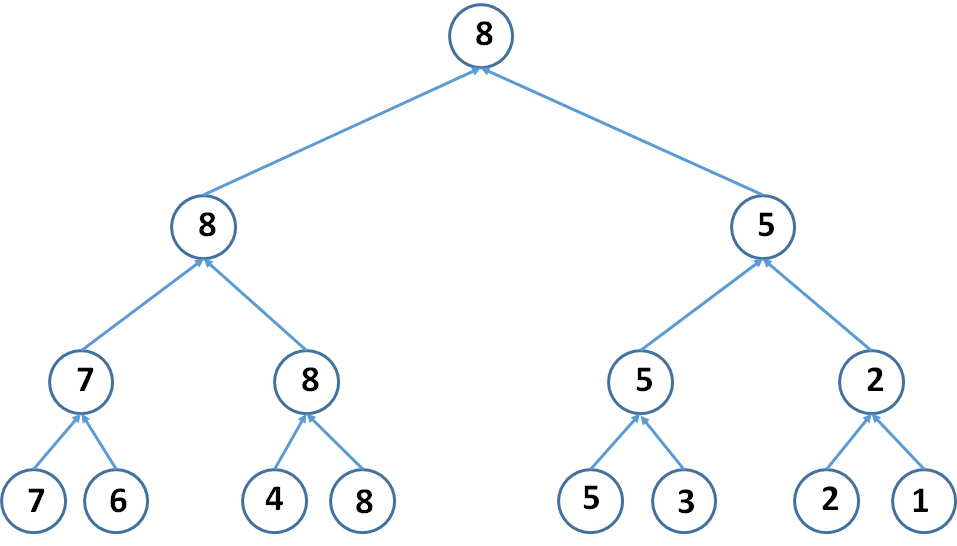
\includegraphics[scale=0.3]{recursiveMaximum.png}
\end{center}

{\bf Analysis:}
\pause
\begin{itemize}
    \item Recurrence Relation: $T(n) = 2T(\frac{n}{2}) + 1 = O(n)$
    \item Number of Comparisons: $n-1$ (Intuition)
\end{itemize}
\end{frame}


\begin{frame}[fragile]{Simultaneous Maximum and Minimum}

{\bf Aim:} Find the maximum and minimum of array $A$ 
\pause
\begin{verbatim}
Minimum-Maximum(A):
    min = Minimum(A)
    max = Maximum(A)
    return min, max
\end{verbatim}
{\bf Analysis:}
\pause
\begin{itemize}
    \item Number of Comparisons: $(n-1)$ + $(n-1)$ = $2n-2$
    \pause
    \item Slightly better: $(n-1)$ + $(n-2)$ = $2n-3$ (for e.g., by swapping min with first element of array)
\end{itemize}
\end{frame}


\begin{frame}{Simultaneous Maximum and Minimum - Visualization}
\begin{center}
    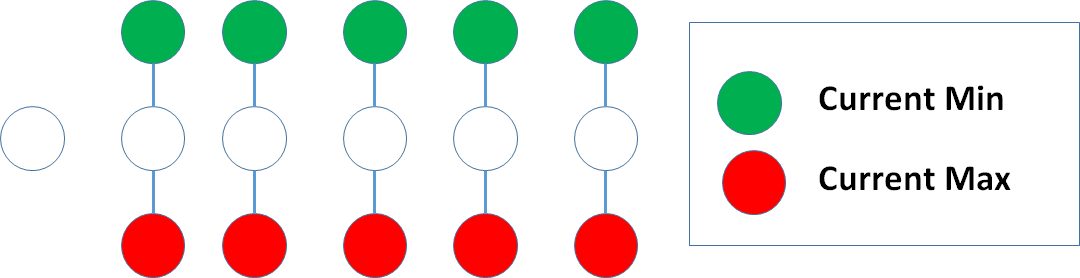
\includegraphics[scale=0.4]{simMinMaxEg1.png}
\end{center}
\end{frame}


\begin{frame}{Simultaneous Maximum and Minimum - Better Algorithm}
\begin{center}
    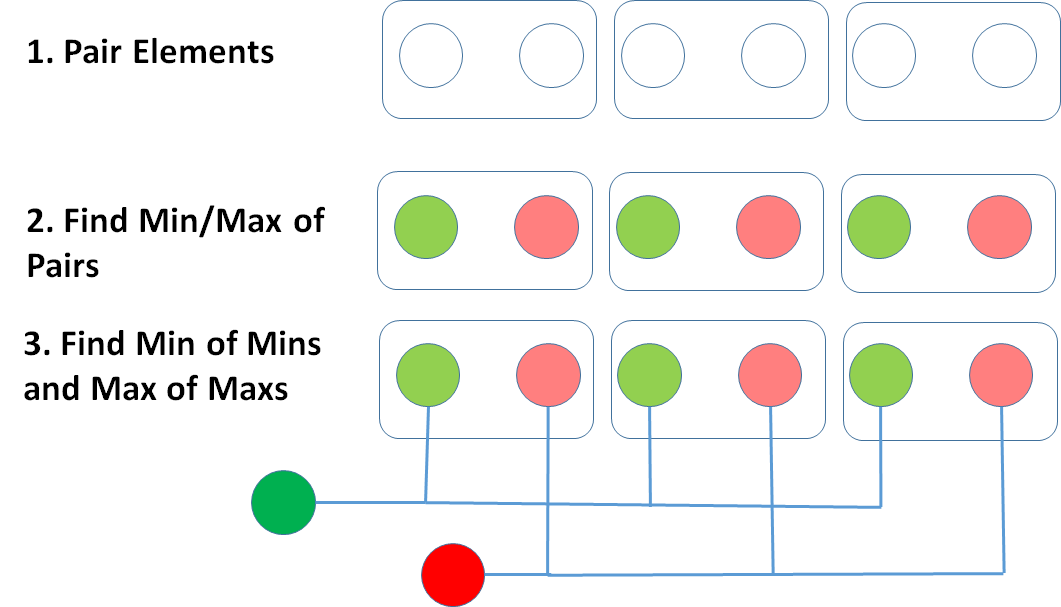
\includegraphics[scale=0.4]{simMinMaxEg2.png}
\end{center}
\end{frame}





\begin{frame}{Simultaneous Maximum and Minimum}

{\bf Analysis:}
\pause
\begin{itemize}
\item Number of Comparisons (approximate): Pairwise + Min of Mins + Max of Maxs
$$(\frac{n}{2}) + (\frac{n}{2}) + (\frac{n}{2})  = \frac{3n}{2}$$
\end{itemize}
\end{frame}




\begin{frame}[fragile]{Finding Second Largest Element - Naive Method}
\pause
\begin{verbatim}
Find-Second-Largest(A):
    max = Maximum(A)
    Swap A[n] with max 
    secondMax = Maximum(A[1:n-1])
    return secondMax
\end{verbatim}
{\bf Analysis:} 
\pause 
\begin{itemize}
\item $n-1$: for finding maximum 
\item $n-2$: for finding 2nd maximum 
\item $2n-3$: total
\end{itemize}

\end{frame}


\begin{frame}[fragile]{Finding Second Largest Element - Tournament Method}
\pause
{\bf Observation:} 
\begin{itemize}
\item In a tournament, second best person could have only be defeated by the best person. 
\item It is not necessarily the other element in the final ``match''
\end{itemize}

\begin{verbatim}
Find-Second-Largest(A):
    max = Recursive-Maximum(A)
    candidates = list of all elements of A that were 
                    directly compared with max
    secondMax = Maximum(candidates)
    return secondMax
\end{verbatim}
\end{frame}


\begin{frame}[fragile]{Finding Second Largest Element - Tournament Method}
\begin{center}
    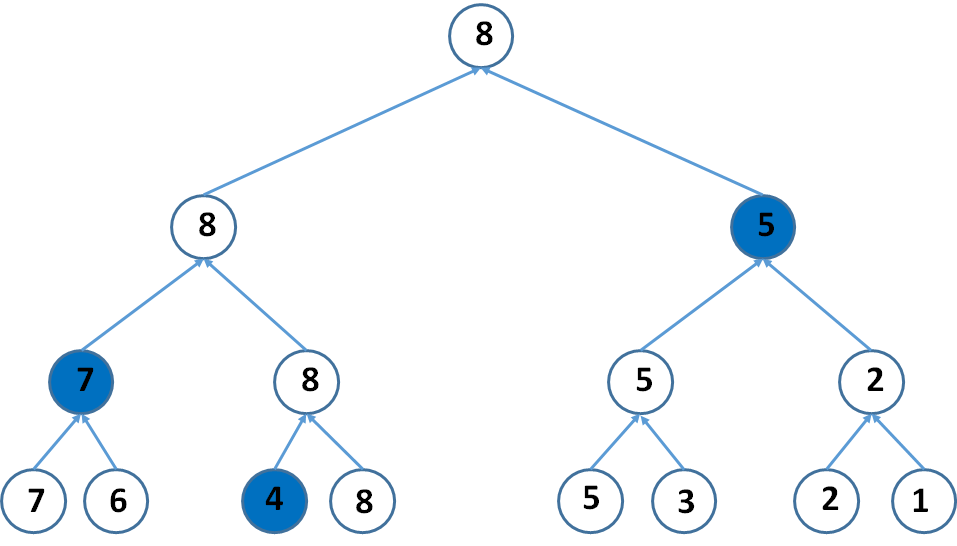
\includegraphics[scale=0.4]{tournamentMethod.png}
\end{center}

{\bf Analysis:} \\
\pause
Number of Comparisons: $ (n-1) + ( \lceil \lg n \rceil - 1) = n +  \lceil \lg n \rceil - 2$
\end{frame}



\begin{frame}{Selection Problem}
\begin{itemize}
\item {\bf Input:} A set $A$ of $n$ (distinct) numbers and an integer $i$ with $1 \leq i \leq n$
\item {\bf Output:} $i^{th}$ smallest element in $A$ 
\item Naive Solution?
\begin{itemize}
    \item Sort $A$ and pick $A[i]$
    \item Time Complexity: $O(n \log n)$
\end{itemize}
\item {\bf Surprising Result}: Can be solved in $O(n)$ time!
\end{itemize}
\end{frame}

\begin{frame}{QuickSelect}
\begin{itemize}
    \item Divide and Conquer Strategy - Ideas?
    \item Called QuickSelect or Randomized-Select
    \item Invented by Tony Hoare
    \item Works excellent in practice
\end{itemize}
\end{frame}

\begin{frame}{QuickSelect - Case 1}
\begin{center}
    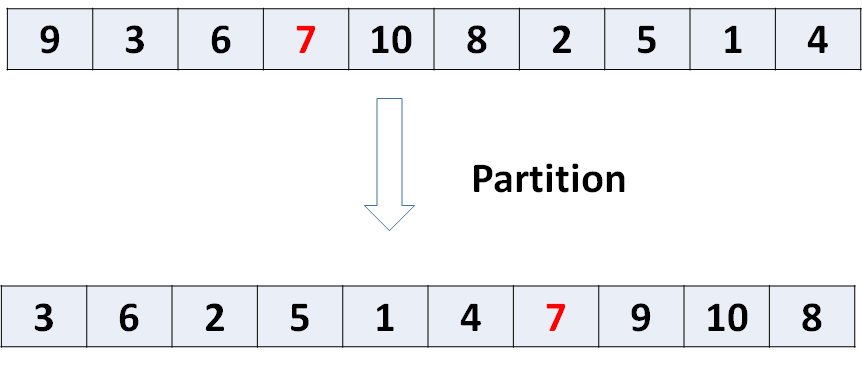
\includegraphics[scale=0.4]{quickSelectCase1.png}
\end{center}
\end{frame}



\begin{frame}{QuickSelect - Case 2}
\begin{center}
    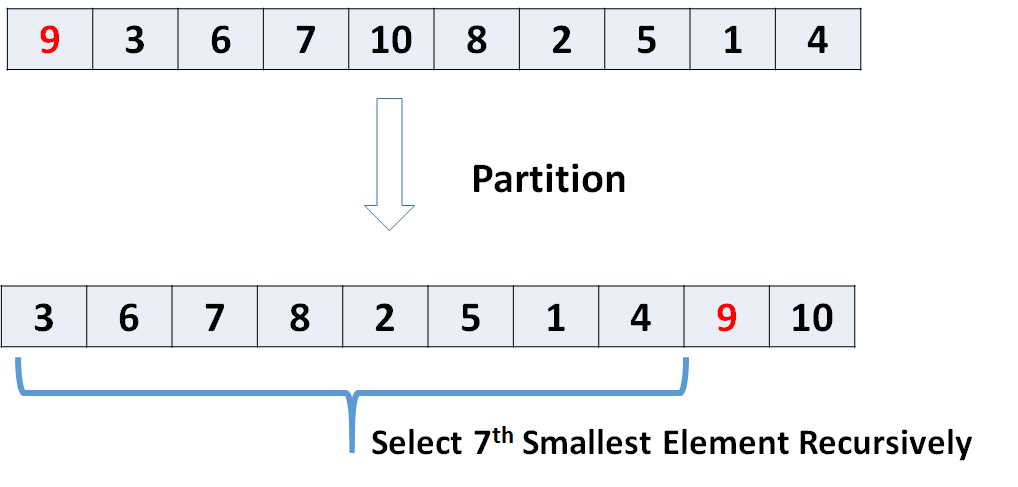
\includegraphics[scale=0.4]{quickSelectCase2.png}
\end{center}
\end{frame}



\begin{frame}{QuickSelect - Case 3}
\begin{center}
    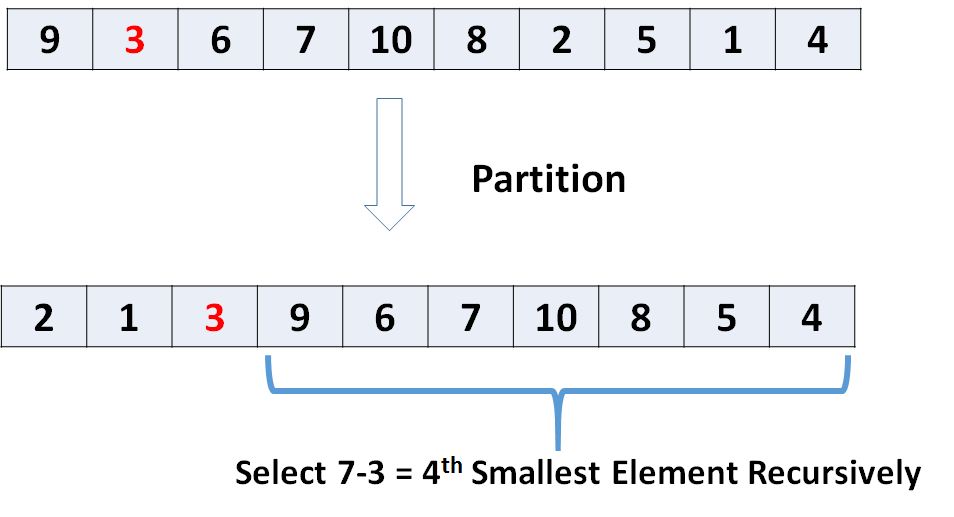
\includegraphics[scale=0.4]{quickSelectCase3.png}
\end{center}
\end{frame}

\begin{frame}[fragile]{QuickSelect PseudoCode}
\begin{verbatim}
Randomized-Select(A, p, r, i)
    if p == r:
        return A[p]
    q = Randomized-Partition(A, p, r)
    k = q - p + 1
    if i == k
        return A[q]
    elseif i < k
        return Randomized-Select(A, p, q-1, i)
    else
        return Randomized-Select(A, q+1, r, i-k)
\end{verbatim}
\end{frame}


\begin{frame}{QuickSelect - Intuition}
\begin{center}
    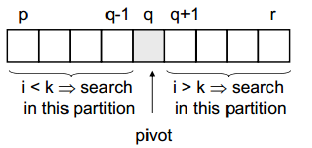
\includegraphics[scale=0.7]{quickSelectSummary.png}
\end{center}
\end{frame}


\begin{frame}{QuickSelect - Analysis}
\begin{itemize}
    \item Recurrence Relation: \pause $$T(n) = T(|L|) + n \text{ or } T(n) = T(|R|) + n$$ 
    \item Best Case: \pause $T(n) = T(\frac{n}{2}) + n$ $\Rightarrow$ $T(n) = O(n)$
    \item Worst Case: \pause $T(n) = T(n-1) + n$ $\Rightarrow$ $T(n) = O(n^2)$
    \begin{itemize}
        \item Worst than sorting !
    \end{itemize}
    \item Lucky Case: (assume a 1:9 split) \pause
    \begin{itemize}
        \item $T(n) = T(\frac{9n}{10}) + n$ $\Rightarrow$ $T(n) = O(n)$
    \end{itemize}
\end{itemize}
\end{frame}



\begin{frame}{QuickSelect and QuickSort}

\tblue{Similarities:}
\pause
\begin{itemize}
    \item Both invented by Tony Hoare 
    \item Both use D\&C and randomization
    \item Best and Average case behavior is good but has bad worst case behavior (same: $O(n^2)$)
    \item Works very well in practice
\end{itemize}

\tblue{Differences:}
\pause
\begin{itemize}
    \item QuickSelect iterates on one partition only while QuickSort on both
    \item Objective: Sorting vs Selection
\end{itemize}
\end{frame}



\begin{frame}{Median of Median Algorithm}
\begin{itemize}
    \item QuickSelect works well in Practice - linear expected time
    \item Worst case is worse than sorting $O(n^2)$
    \item Can we solve Selection problem in worst case Linear time?
    \pause
    \begin{itemize}
        \item Yes!
        \item Designed by Blum, Floyd, Pratt, Rivest \& Tarjan in 1973
        \item Basic Idea: Identify a good pivot so that partition is ``balanced''
        \item Aka ``Median of Median'' or ``Worst case Linear time Order Statistics''
    \end{itemize}
\end{itemize}
\end{frame}



\begin{frame}{Median of Median Algorithm}

\tblue{SELECT(A, i, n):}
\begin{enumerate}
    \item Divide $n$ elements into groups of $5$. Last group might have less than $5$ elements
    \item Sort each group insertion sort. Find the median of each group
    \item Use SELECT recursively to find median $x$ of the $\lfloor \frac{n}{5} \rfloor$ medians
    \item Partition $A$ around $x$. Let position $x$ be $k$ 
    \item If $i=k$ then return $x$
    \item If $i < k$, use SELECT recursively on the low side to find $i^{th}$ smallest element
    \item If $i > k$, use SELECT recursively on the high side to find $(i-k)^{th}$ smallest element 
\end{enumerate}

\end{frame}



\begin{frame}{Median of Median - Visualization\footnote{\url{http://www.cs.gmu.edu/~ashehu/sites/default/files/cs583/ShehuLecture04.pdf}}}
\begin{center}
    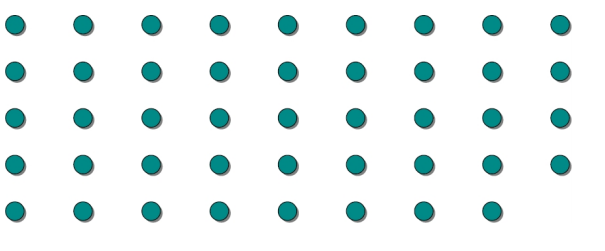
\includegraphics[scale=0.4]{medianOfMedian1.png}
\end{center}
\begin{itemize}
    \item Original input array $A$ with $n$ elements 
\end{itemize}
\end{frame}


\begin{frame}{Median of Median - Visualization\footnote{\url{http://www.cs.gmu.edu/~ashehu/sites/default/files/cs583/ShehuLecture04.pdf}}}
\begin{center}
    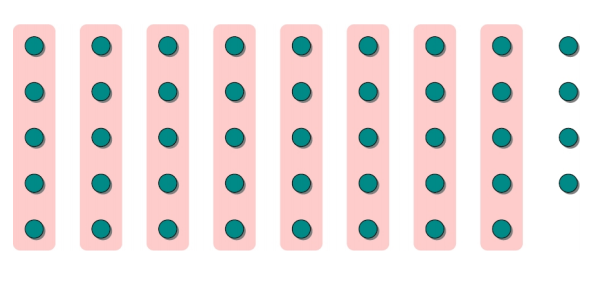
\includegraphics[scale=0.4]{medianOfMedian2.png}
\end{center}
\begin{itemize}
    \item Step 1: Divide $A$ into groups of $5$ 
\end{itemize}
\end{frame}




\begin{frame}{Median of Median - Visualization\footnote{\url{http://www.cs.gmu.edu/~ashehu/sites/default/files/cs583/ShehuLecture04.pdf}}}
\begin{center}
    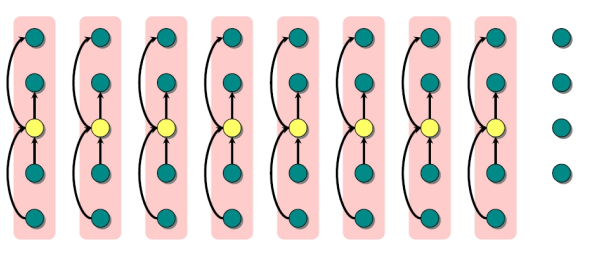
\includegraphics[scale=0.4]{medianOfMedian3.png}
\end{center}
\begin{itemize}
    \item Step 2: Sort each group by Insertion sort. Find its median.
    \item $A \rightarrow B$ means $A > B$
\end{itemize}
\end{frame}




\begin{frame}{Median of Median - Visualization\footnote{\url{http://www.cs.gmu.edu/~ashehu/sites/default/files/cs583/ShehuLecture04.pdf}}}
\begin{center}
    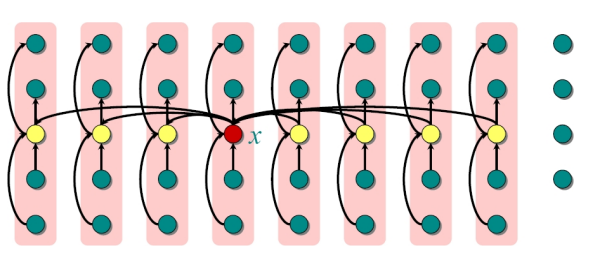
\includegraphics[scale=0.4]{medianOfMedian4.png}
\end{center}
\begin{itemize}
    \item Step 3: Use SELECT recursively to find median $x$ of the $\lfloor \frac{n}{5} \rfloor$ medians. 
    \item $A \rightarrow B$ means $A > B$
\end{itemize}
\end{frame}




\begin{frame}{Median of Median - Visualization\footnote{\url{http://www.cs.gmu.edu/~ashehu/sites/default/files/cs583/ShehuLecture04.pdf}}}
\begin{center}
    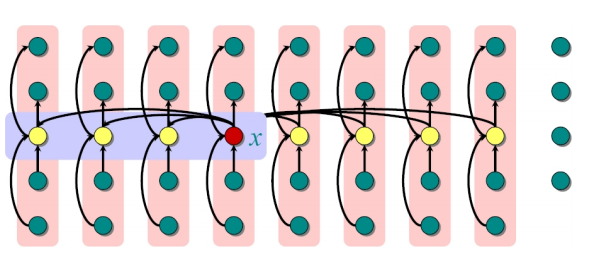
\includegraphics[scale=0.4]{medianOfMedian5.png}
\end{center}
\begin{itemize}
    \item Question: How many medians are less than $x$? \pause
    \item At least half of the group medians are $\leq x$
    \item So at least $\lfloor \lfloor \left( \frac{n}{5} \right) / 2 \rfloor \rfloor$  = $\lfloor \frac{n}{10} \rfloor$
\end{itemize}
\end{frame}




\begin{frame}{Median of Median - Visualization\footnote{\url{http://www.cs.gmu.edu/~ashehu/sites/default/files/cs583/ShehuLecture04.pdf}}}
\begin{center}
    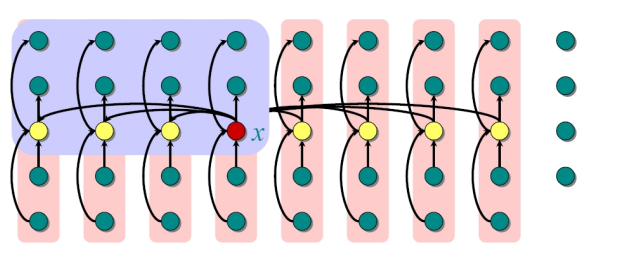
\includegraphics[scale=0.4]{medianOfMedian6.png}
\end{center}
\begin{itemize}
    \item Question: How many elements in  $A$ are {\bf smaller} i.e. $\leq x$? \pause
    \item All elements smaller than the medians that were in turn smaller than $x$ 
    \begin{itemize}
        \item $\lfloor \frac{n}{10} \rfloor$ medians were $\leq x$
        \item So, $\lfloor \frac{3n}{10} \rfloor$ elements in $A$ are $\leq x$
    \end{itemize}
\end{itemize}
\end{frame}




\begin{frame}{Median of Median - Visualization\footnote{\url{http://en.wikipedia.org/wiki/Median_of_medians}}}
\begin{center}
    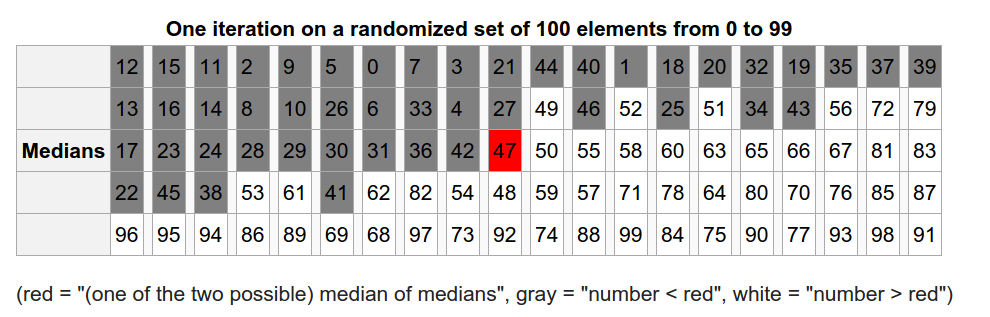
\includegraphics[scale=0.32]{medianOfMedianWiki.png}
\end{center}
\begin{itemize}
    \item Note that some elements such as $22, 45, 38, 41$ are smaller than $x$
    \item But we don't count them as we are not sure
\end{itemize}
\end{frame}




\begin{frame}{Median of Median - Visualization\footnote{\url{http://www.cs.gmu.edu/~ashehu/sites/default/files/cs583/ShehuLecture04.pdf}}}
\begin{center}
    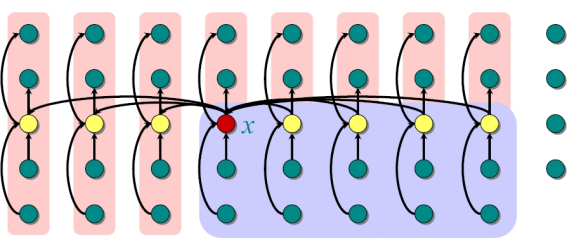
\includegraphics[scale=0.4]{medianOfMedian7.png}
\end{center}
\begin{itemize}
    \item Question: How many elements in  $A$ are {\bf larger} i.e. $\geq x$? \pause
    \item All elements larger than the medians that were in turn $\geq x$ 
    \begin{itemize}
        \item $\lfloor \frac{n}{10} \rfloor$ medians were $\geq x$
        \item So, $\lfloor \frac{3n}{10} \rfloor$ elements in $A$ are $\geq x$
    \end{itemize}
\end{itemize}
\end{frame}



\begin{frame}{Median of Median Algorithm - Analysis}

\tblue{SELECT(A, i, n):}
\begin{enumerate}
    \item Divide $n$ elements into groups of $5$. Last group might have less than $5$ elements
    \item Sort each group insertion sort. Find the median of each group
    \item Use SELECT recursively to find median $x$ of the $\lfloor \frac{n}{5} \rfloor$ medians
    \item Partition $A$ around $x$. Let position $x$ be $k$ 
    \item If $i=k$ then return $x$
    \item If $i < k$, use SELECT recursively on the low side to find $i^{th}$ smallest element
    \item If $i > k$, use SELECT recursively on the high side to find $(i-k)^{th}$ smallest element 
\end{enumerate}

\end{frame}


\begin{frame}{Median of Median Algorithm - Analysis}
\begin{itemize}
    \item Line 1: \pause $O(n)$ 
    \item Line 2: \pause $\frac{n}{5} \times c_1 = O(n)$. 
    \begin{itemize}
        \item Sorting 5 elements requires constant $c_1$ comparisons 
    \end{itemize}
    \item Line 3: \pause $T(\frac{n}{5})$
    \item Line 4: \pause $T(n)$
    \item Line 5-7: \pause Worst Case Analysis : $T(\frac{3n}{4})$
    \item Size of largest partition: $(n - \lfloor \frac{3n}{10} \rfloor) =  \lfloor \frac{7n}{10} \rfloor$
    \item But for $n \geq 50$, we have $\lfloor \frac{3n}{10} \rfloor \geq \frac{n}{4}$
    \item So, size of largest partition is $(n - \frac{n}{4}) = \frac{3n}{4}$
    \item {\bf Final recurrence:} $T(n) = T(\frac{n}{5}) + O(n) + T(\frac{3n}{4})$
    \item {\bf Solution :} $O(n)$
\end{itemize}
\end{frame}



\begin{frame}{Median of Median - Conclusions}
\begin{itemize}
    \item Even though the algorithm is $O(n)$ (asymptotically linear), it has a huge {\em hidden} constant
    \item So, in practice, it runs much slower
    \item Use QuickSelect in practice
    \item To think about: What happens when we divide them into 
    \begin{itemize}
        \item Groups of $7$?
        \item Groups of $3$?
    \end{itemize}
\end{itemize}
\end{frame}



\begin{frame}{Selection Problem - Applications}
\begin{itemize}
    \item  Note: SELECT algorithm is a general purpose algorithm 
    \begin{itemize}
        \item Can solve Selection problem for any $i$ (not just the median)
    \end{itemize}
    \item How to find the $i^{th}$ {\bf largest}? \pause
    \begin{itemize}
        \item Call SELECT to find $(n-i+1)^{th}$ smallest element
    \end{itemize}
    \item How to find median? \pause
    \begin{itemize}
        \item Call SELECT with $i=\lfloor \frac{n+1}{2} \rfloor$
        \item By convention, lower median is chosen for even sized sets 
    \end{itemize}
\end{itemize}
\end{frame}



\begin{frame}{Finding Majority}
\begin{itemize}
    \item {\bf Majority:} The majority of a set of numbers is defined as a number that repeats at least $\frac{n}{2}$ times in the set.
    \item {\bf Problem:} Find majority of a set $A$ {\bf if} one exists.
    \item {\bf Naive Algorithm:} \pause 
        \begin{itemize}
            \item Sort and check if it has a majority element: $O(n \lg n)$
        \end{itemize}
    \item {\bf Better Algorithm:} \pause
    \begin{itemize}
        \item Use QuickSelect to find Median $m$
        \item Partition $A$ around median $m$
        \item Verify if median is the majority element
        \item Why does it work?
    \end{itemize}
    \item {\bf Time Complexity:} $O(n) + n + n = O(n)$
\end{itemize}
\end{frame}


\begin{frame}{Finding Majority - Visualization}
\begin{center}
    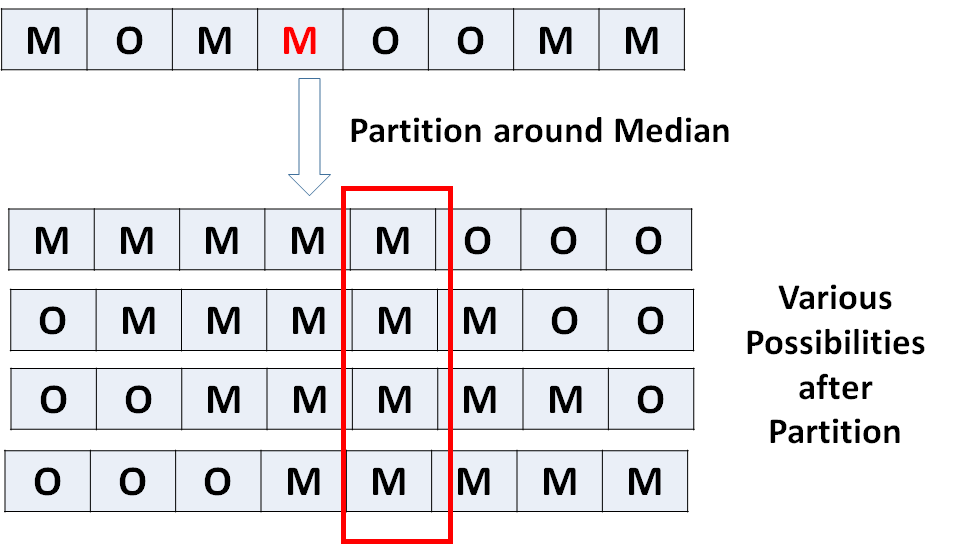
\includegraphics[scale=0.4]{findingMajorityVisualization.png}
\end{center}
\end{frame}


\begin{frame}{Finding Majority - Boyer-Moore Algorithm}
\begin{itemize}
    \item Boyer-Moore: one pass algorithm to find Majority candidate
    \begin{itemize}
        \item Don't confuse it with Boyer-Moore String Search algorithm
    \end{itemize}
    \item {\bf Algorithm:}
    \begin{itemize}
        \item Maintain current candidate (initially None) and a counter (initially 0).
        \item Sweep the array from left to right
        \item When we move the pointer forward over an element $e$:
        \begin{itemize}
            \item If the counter is $0$, we set the current candidate to $e$ and we set the counter to $1$.
            \item If the counter is not 0, we increment the counter if $e$ is the current candidate.
            \item If the counter is not 0, we decrement the counter if $e$ is not the current candidate.
        \end{itemize}
    \end{itemize}
    \item Visualization: \url{http://www.cs.utexas.edu/~moore/best-ideas/mjrty/example.html}
\end{itemize}
\end{frame}

\begin{frame}{Finding Mode}
\begin{itemize}
    \item {\bf Mode:} The mode of a set of numbers is the element that occurs most often. 
    \item {\bf Algorithm:} Sort and find the longest sequence $O(n \lg n)$.
\end{itemize}
\end{frame}


\begin{frame}{Summary}

\tblue{Major Concepts:}
\begin{itemize}
\item Concept of Order Statistics and Rank
\item Popular Order Statistics - Min, Max, Median
\item Selection Problem
\item Mode and Majority
\item Cool, non-obvious algorithms for even the simplest problems!
\end{itemize}
\end{frame}


\end{document}

